% --- First Plot: Frequency Response ---
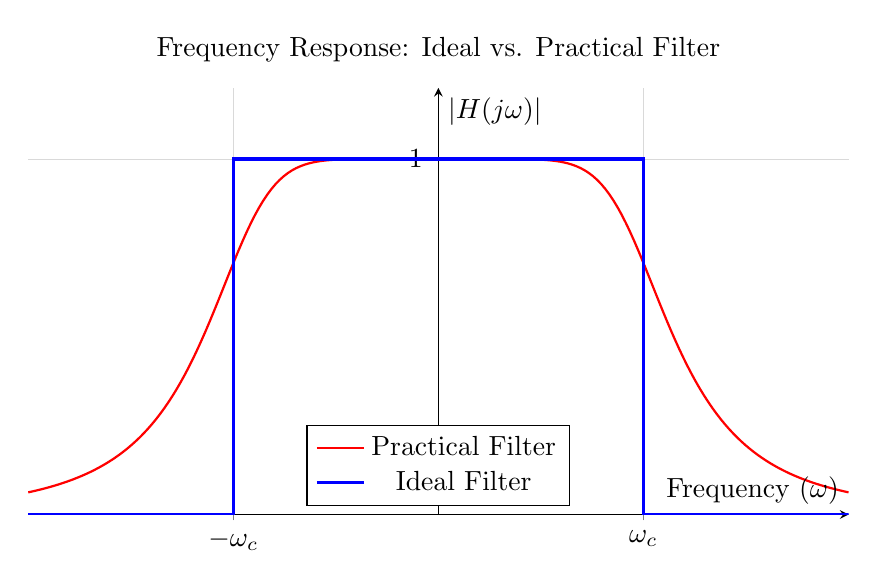
\begin{tikzpicture}
	\begin{axis}[
		width=12cm,
		height=7cm,
		title={Frequency Response: Ideal vs. Practical Filter},
		xlabel={Frequency ($\omega$)},
		ylabel={$|H(j\omega)|$},
		axis lines=middle,
		xmin=-5, xmax=5,
		ymin=0, ymax=1.2,
		xtick={-2.5, 2.5},
		xticklabels={$-\omega_c$, $\omega_c$},
		ytick={1},
		grid=major,
		grid style={line width=.1pt, draw=gray!30},
		legend style={at={(0.5,0.02)}, anchor=south},
		]
		
		% Practical Filter (Butterworth-like magnitude)
		\addplot[red, thick, domain=-5:5, samples=200, mark=none]
		{1/(sqrt(1+(x/2.5)^8))};
		\addlegendentry{Practical Filter};
		
		% Ideal Filter (brick-wall)
		\addplot[blue, very thick, mark=none]
		coordinates {(-5,0) (-2.5,0) (-2.5,1) (2.5,1) (2.5,0) (5,0)};
		\addlegendentry{Ideal Filter};
		
	\end{axis}
\end{tikzpicture}

% --- Second Plot: Impulse Response (Corrected and Refactored) ---
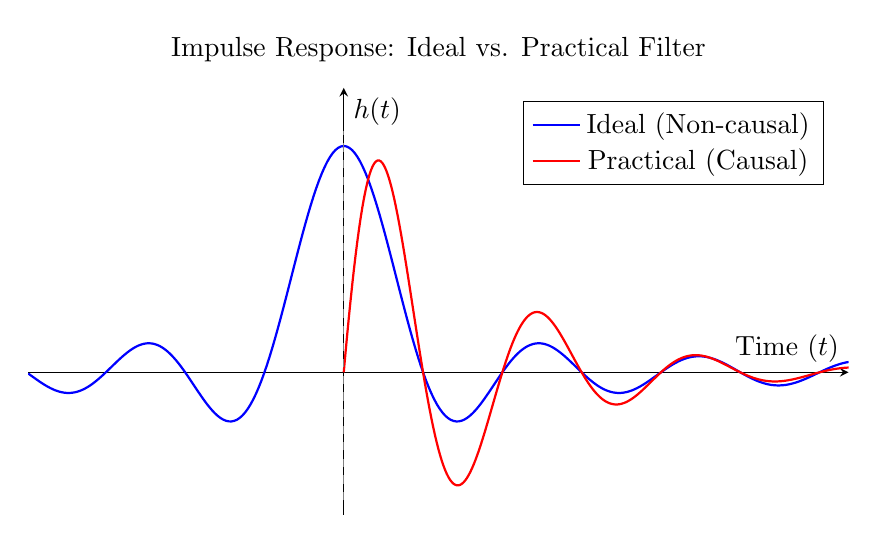
\begin{tikzpicture}
	\begin{axis}[
		width=12cm,
		height=7cm,
		title={Impulse Response: Ideal vs. Practical Filter},
		xlabel={Time ($t$)},
		ylabel={$h(t)$},
		axis lines=middle,
		xmin=-5, xmax=8,
		ymin=-0.5, ymax=1.0,
		xtick={0},
		ytick=\empty,
		grid=major,
		grid style={line width=.1pt, draw=gray!30},
		legend pos=north east,
		% Declare a radian-based sinc function for robustness and clarity.
		% This function computes sin(x)/x, handling the case at x=0.
		declare function={
			sincrad(\x) = (\x==0) ? 1 : sin(\x r)/\x;
		},
		]
		
		% Ideal impulse response is h(t) = (omega_c/pi) * sinc(omega_c*t)
		% With omega_c = 2.5, we plot (2.5/pi) * sincrad(2.5*t)
		\addplot[blue, thick, domain=-5:8, samples=300, mark=none]
		{ (2.5/pi) * sincrad(2.5*x) };
		\addlegendentry{Ideal (Non-causal)};
		
		% Practical impulse response (causal, damped sinusoid)
		\addplot[red, thick, domain=0:8, samples=300, mark=none]
		{exp(-0.5*x)*sin(deg(2.5*x))};
		\addlegendentry{Practical (Causal)};
		
		% Vertical line at t=0 to emphasize causality
		\draw[dashed, gray] (axis cs:0,-0.45) -- (axis cs:0,0.85);
		
	\end{axis}
\end{tikzpicture}








